\documentclass[12pt,a4paper]{article}
\usepackage[utf8]{inputenc}
\usepackage[english]{babel}
\usepackage{amssymb}%usar formula matematica
\usepackage{graphicx}%insere imagem
\usepackage{wrapfig}
\usepackage{float}
\usepackage{hyperref}
\usepackage{indentfirst}
\usepackage{enumitem}
\usepackage{amsmath}
\usepackage{booktabs}
\usepackage{amssymb}
\usepackage{cancel}
\usepackage{subfig}
\usepackage{multirow}
\usepackage{siunitx}
\usepackage[alf]{abntex2cite} 
%\newtheorem{teo}{Teorema}
\renewcommand{\baselinestretch}{1.5}%estilo da fonte
\usepackage{verbatim} % para comentarios
\usepackage{float}  % para imagens
\usepackage{geometry}%configura margem
%\geometry{verbose,a4paper,tmargin=30mm,bmargin=20mm,lmargin=30mm,rmargin=20mm}

\usepackage{listings}
\usepackage{xcolor}

\definecolor{codegreen}{rgb}{0,0.6,0}
\definecolor{codegray}{rgb}{0.5,0.5,0.5}
\definecolor{codepurple}{rgb}{0.58,0,0.82}
\definecolor{backcolour}{rgb}{0.95,0.95,0.92}

\lstdefinestyle{mystyle}{
    backgroundcolor=\color{backcolour},   
    commentstyle=\color{codegreen},
    keywordstyle=\color{magenta},
    numberstyle=\tiny\color{codegray},
    stringstyle=\color{codepurple},
    basicstyle=\ttfamily\footnotesize,
    breakatwhitespace=false,         
    breaklines=true,                 
    captionpos=b,                    
    keepspaces=true,                 
    numbers=left,                    
    numbersep=5pt,                  
    showspaces=false,                
    showstringspaces=false,
    showtabs=false,                  
    tabsize=2
}

\lstset{style=mystyle}

\begin{document}
\newgeometry{top = 1.5cm, lmargin = 1.5cm, rmargin = 1.5cm} 

\begin{figure}[H]
	\centering
	\begin{minipage}[]{0.07\linewidth}
	
\includegraphics[width=\linewidth]{images/ufop.png}	
	\end{minipage}
\hfill
	\begin{minipage}[]{0.6\linewidth}
		\centering
	\textbf{UNIVERSIDADE FEDERAL DE OURO PRETO\\}
		Rafael Francisco de Oliveira - 2021.10171\\
		PCC104 - Projeto e Análise de Algoritmos\\
		Github: \href{https://github.com/raffoliveira/Master_Degree}{raffoliveira}\\
		Lista 4
		
	\end{minipage}
\hfill	
	\begin{minipage}[c]{0.15\linewidth}
	
\includegraphics[width=\linewidth]{images/icea.jpg}	
	\end{minipage}

\vspace{0.5cm}
\hrulefill
\end{figure}

{\Large \textbf{Questões práticas}}

\vspace{0.5cm}

A pasta denominada \textsf{lista\_4} no GitHub contém os respectivos exercícios da lista. A implementação dos algoritmos foi dividida em módulos. Abaixo segue a uma breve descrição dos arquivos disponibilizados:

\begin{itemize}
	\item A pasta \textsf{exercicios} contém os arquivos de cada exercício.
	\item O arquivo chamado \textsf{functions.h} é responsável por ter as implementações de todas as funções e importação de bibliotecas. 
	\item A pasta \textsf{testes} contém os arquivos contendo as instâncias para testes. Para a escolha de cada arquivo nesta pasta, basta modificar as linhas \textsf{85} e \textsf{87} do arquivo \textsf{functions.h}  para o tipo \textsf{float} e as linhas \textsf{112} e \textsf{114} do arquivo \textsf{functions.h}  para o tipo \textsf{string}, as quais especificam o caminho do diretório da pasta e o nome do arquivo escolhido, respectivamente. 
\end{itemize}

Para a execução dos algoritmos, execute os seguintes comandos abaixo no terminal, mudando apenas o nome do exercício desejado:

\begin{table}[H]
	\centering
	\begin{tabular}{|l|}
		\hline
		\textbf{g++ exercicio\_1.cpp -o exe}\\		
		\textbf{./exe}\\
		\hline
	\end{tabular}
\end{table}

O primeiro comando irá compilar o código e gerar um arquivo executável nomeado de acordo com nome especificado no comando. No exemplo acima, o executável seria renomeado como \textit{exe}. Para executar o executável, basta executar a segunda linha do comando acima especificando o nome do executável criado.


\newpage

{\Large \textbf{Exercícios}}

\vspace{0.5cm}

\textbf{Exercício 2)} 

\begin{figure}[H]
    \centering
    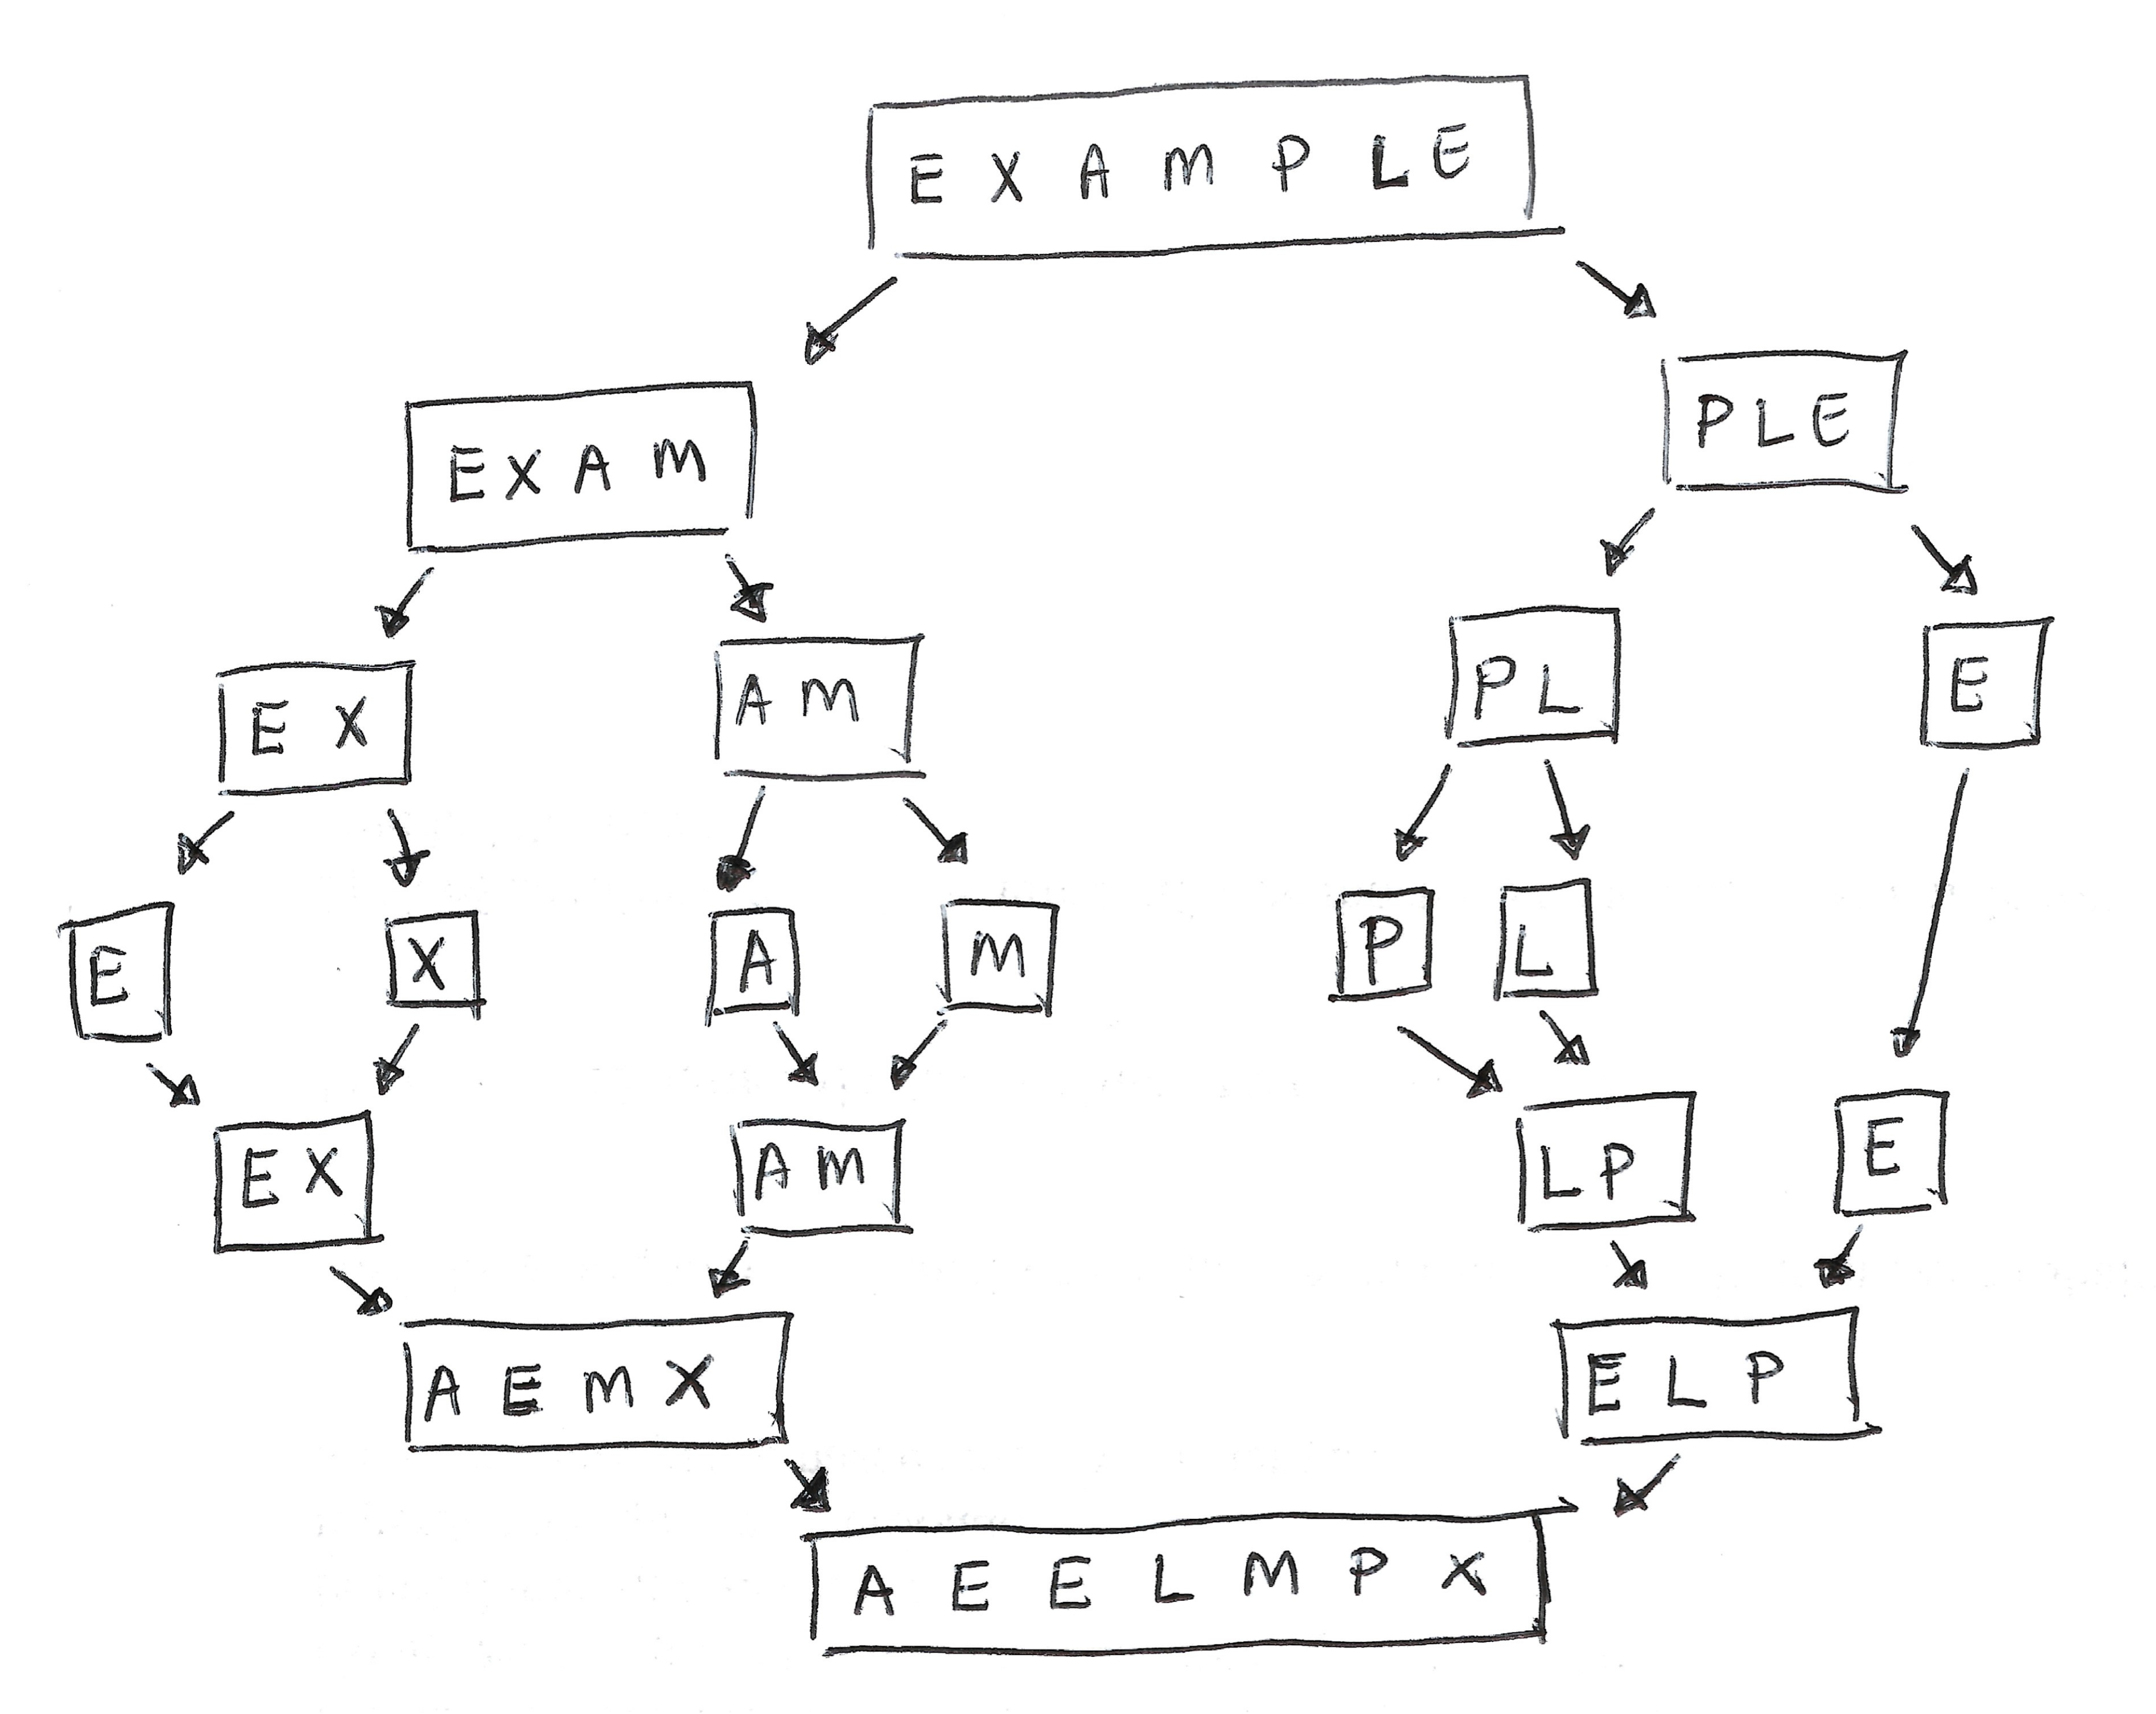
\includegraphics[width=\textwidth]{images/exe2.pdf}
\end{figure}

\hrulefill

\textbf{Exercício 3)} 

Na maioria de suas implementações (iterativas e recursivas), o \emph{mergesort} é estável. Segundo a definição formal, um algoritmo de ordenação é estável se, e somente se, para todo par de dados $x$ e $y$, se antes da ordenação $x$ aparece antes de $y$ (índice menor) e a chave de $x$ for igual à chave de $y$, então após a ordenação $x$ continuará antes de $y$. Logo, se dois elementos são iguais mas com chaves diferentes, a ordenação tem que levar em consideração a ordem em que aparecem no conjunto original. Abaixo segue um exemplo para ilustrar a ideia.

\begin{center}
    $A = \{f, j, a1, a2, j1\} \longrightarrow$ ordenação $ \longrightarrow A = \{a1, a2, f, j, j1\} $ 
\end{center}

Pode-se observar que os elementos $a1$ aparece antes do elemento $a2$ e $j$ aparece antes do elemento $j1$. No conjunto ordenado, essa ordem permanece.

\hrulefill

\textbf{Exercício 4)} 

\textbf{a)} 

Não irá atrapalhar, pois na divisão do arranjo, o maior valor sempre irá retornar de acordo com as subdivisões não importando se há vários elementos iguais.

\textbf{b)}

$T(n) = 2T\left(\dfrac{n}{2}\right) + 2$ para $T(2)=1$. Considerando $n =2^k$\\

\begin{table}[h]
    \centering
    \begin{tabular}{ll}
        $T(n) = 2T(2^{k-1}) + 2$ & $T(2^{k-i}) = T(2) \longrightarrow 2^{k-i} = 2 \longrightarrow i = k-1$\\
        $T(n) = 2(2T(2^{k-2})+2) + 2$ & $T(n) = 2^{k-1}T(2) + 2^k - 2$\\
        $T(n) = 2(2(2T(2^{k-3})+2)+2) + 2$ & $T(n) = 2^{k-1} + 2^k - 2$\\
        $T(n) = 8(T(2^{k-3}))+14$ & $T(n) = \dfrac{2^k}{2} + 2^k - 2$\\
        $T(n) = 2^i(T(2^{k-i}))+2^{i+1}-2$ & $T(n) = \dfrac{n}{2} + n - 2 \longrightarrow \dfrac{3n}{2} - 2$\\
    \end{tabular}
\end{table}

\textbf{c)}

Realizando a análise do algoritmo de força bruta, percebe-se que dentro do laço \emph{for}, há duas comparações (operação básica). Como o laço percorre todo o vetor de tamanho ($n$) menos um o primeiro elemento, a complexidade do mesmo é $2(n-1) = 2n-2$. Logo, o algoritmo que utiliza o paradigma ``dividir e conquistar'' é $25\%$ mais rápido do que o de força bruta.

\lstinputlisting[language=C++]{minMaxBF.cpp}

\hrulefill

\textbf{Exercício 5)} 

\textbf{a)} 

A relação de recorrência ficou semelhante ao exercício 4.

Logo, $T(n) = 2T\left(\dfrac{n}{2}\right) + 2$ para $T(2)=1$ e considerando $n =2^k$ temos $\dfrac{3n}{2} - 2$.\\

\textbf{b)} 

A relação também ficou semelhante ao exercício 4 como $2(n-1) = 2n-2$. Logo, o algoritmo que utiliza o paradigma ``dividir e conquistar'' é $25\%$ mais rápido do que o de força bruta.

\lstinputlisting[language=C++]{minMaxBFPosition.cpp}

\hrulefill

\textbf{Exercício 7)} 

\begin{figure}[H]
    \centering
    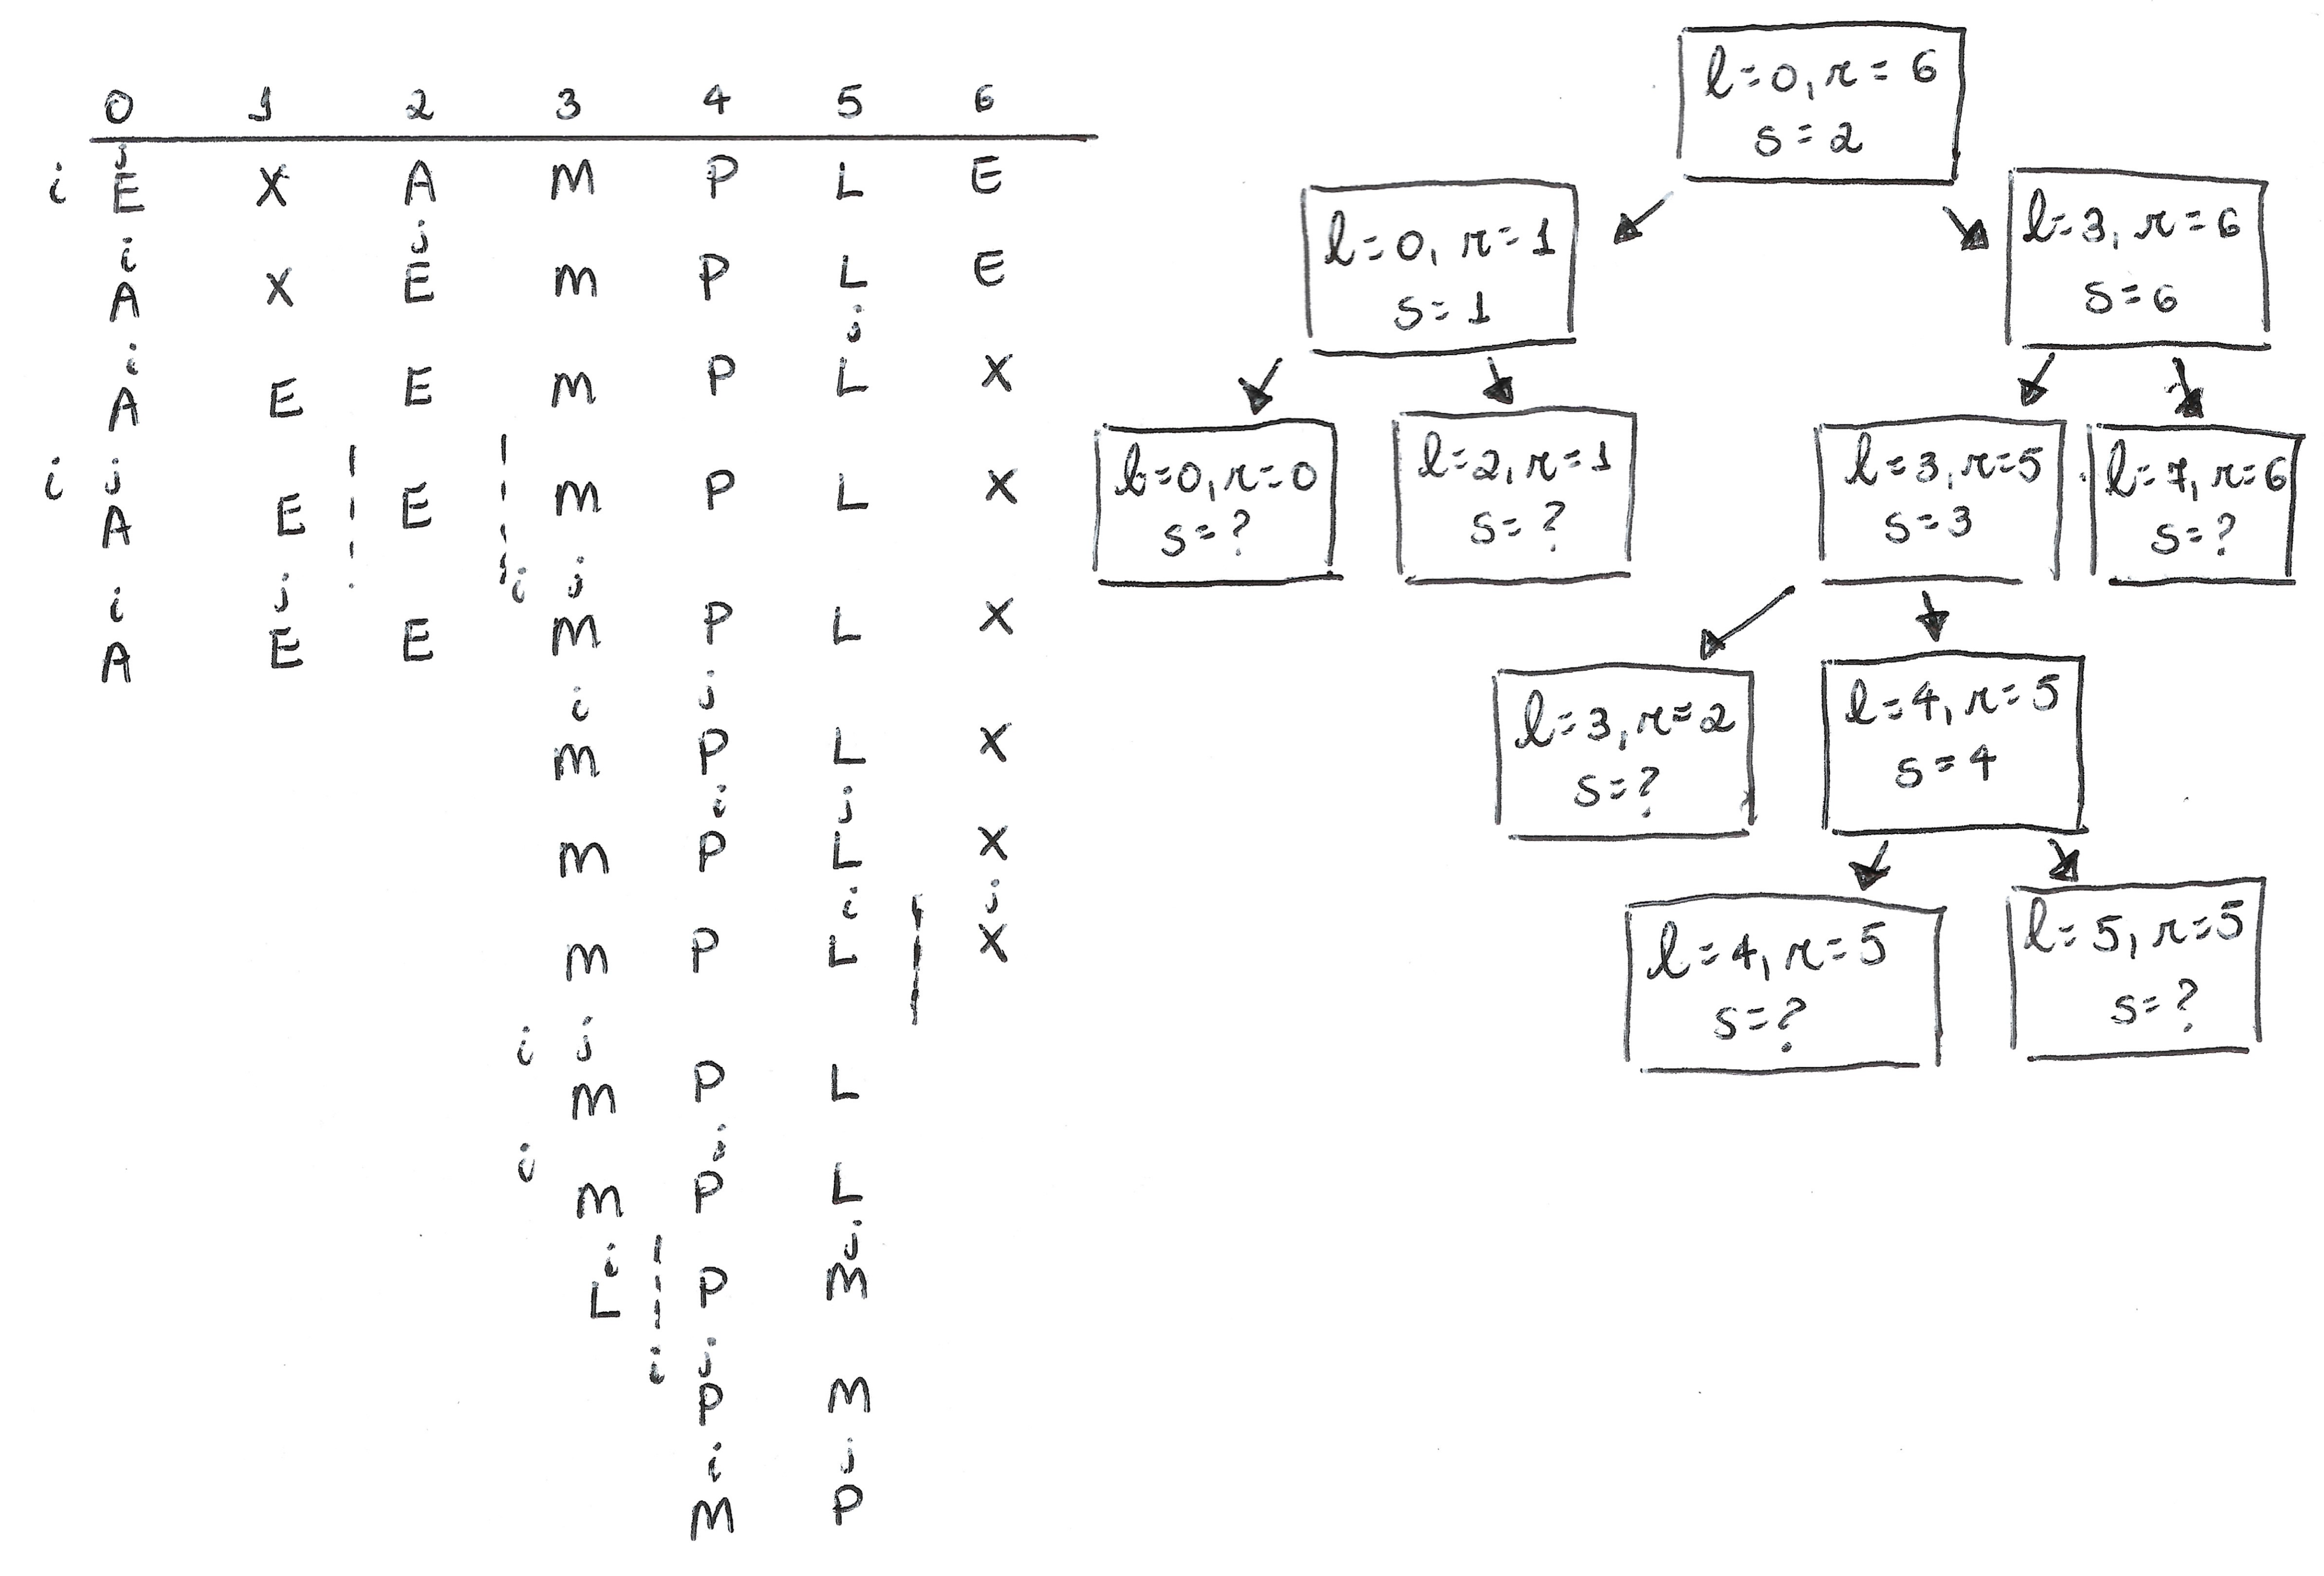
\includegraphics[width=\textwidth]{images/exe7.pdf}
\end{figure}

\hrulefill

\textbf{Exercício 8)} 

Pelo exemplo dado, percebe-se que o elemento $(1,5)$ e  $(1,2)$ foram ordenados sem levar em consideração a precedência do conjunto original. Isso acontece pois o quickSort utiliza um pivot particionar o arranjo.

\begin{figure}[H]
    \centering
    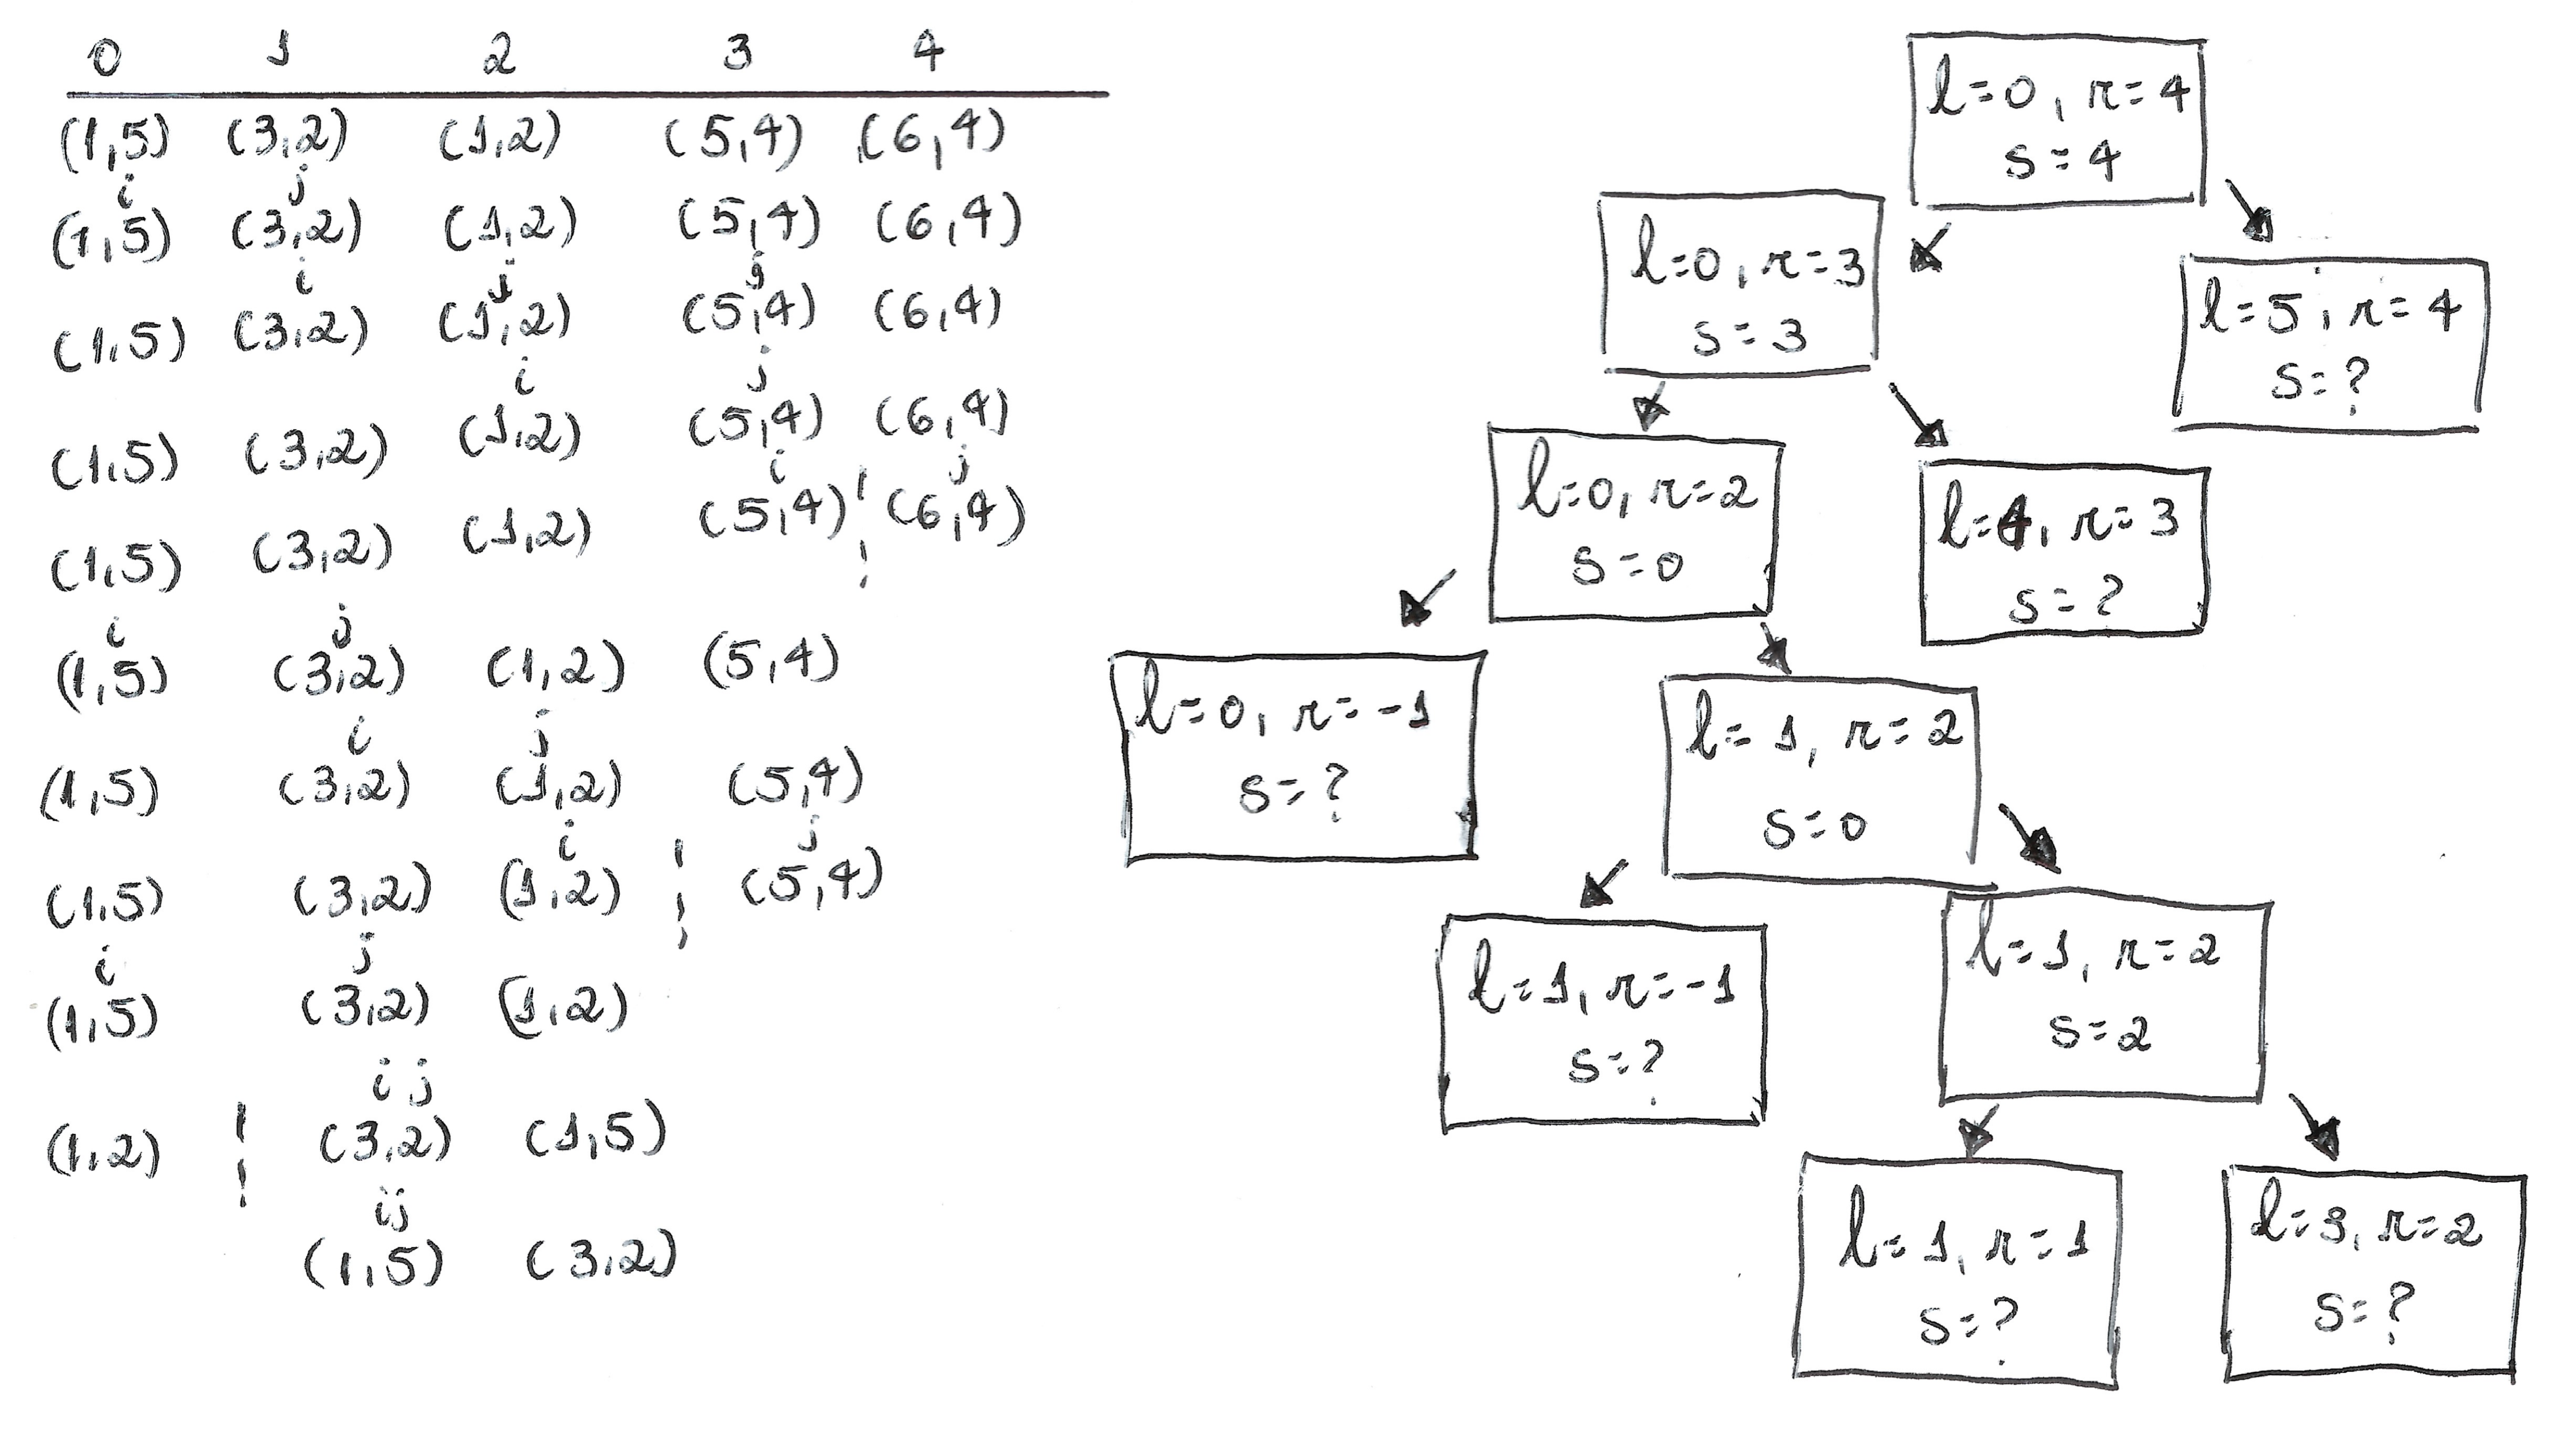
\includegraphics[width=\textwidth]{images/exe8.pdf}
\end{figure}

\hrulefill

\textbf{Exercício 11)}

Preorder= $a\rightarrow b\rightarrow d\rightarrow e\rightarrow c\rightarrow f$

Inorder= $d\rightarrow b\rightarrow e\rightarrow a\rightarrow c\rightarrow f$

Postorder= $d\rightarrow e\rightarrow b\rightarrow f\rightarrow c\rightarrow a$

\hrulefill

\textbf{Exercício 13)}

Analisando a complexidade de cada algoritmo, temos que o algoritmo de Strassen tem complexidade de $n^{2.807}$ enquanto que o algoritmo de força bruta tem complexidade de $n^3$. Logo, o algoritmo de Strassen é 6.5\% mais rápido do que o força bruta.

\hrulefill

\textbf{Exercício 14)}

Analisando a complexidade de cada algoritmo, temos que o algoritmo do \emph{convex hull} por força bruta tem complexidade de $n^3$ enquanto que o algoritmo \emph{quick hull} tem complexidade de $n^2$ no pior caso e $n*log n$ no melhor caso. Logo, o algoritmo \emph{quick hull} é aproximadamente 33\% mais rápido do que o força bruta.

\end{document}

